\chapter{Framework Evaluation and Results}



We need to evaluate the performance of the framework. We will mainly focus our tests on the clustering of authors and the influence of different combinations of rules and parameters on the results. Proper clustering results in a collection of publications related to one author, allowing to define specialties and the level of expertise. 

In order to accomplish realistic and useful results, it's important the tests resemble realistic use-cases. This means testing against both general and borderline queries. Parameters making it easier in disambiguation are rare and country specific author names, a multitude of publications which are written with the same co-authors or the inclusion of the same email address. A combination of these parameters allows for easier manual checking of results, but is consequently less challenging. 

Borderline cases make more defiant evalutations. Author names containing foreign characters or accents make it easier to be misspelled. In contrast, common last names also make it harder to differentiate between different authors. Examples are Anderson or Smith in United States, Chen or Lee in East Asian countries or Peters in Belgium.

% Wat moeten we bespreken in dit hoofdstuk:

% De testopstelling
	% Hoe zit deze in elkaar
	% Waarom hebben hiervoor gekozen
	% Vergelijking met anderen?
% De bekomen resultaten
% (Vergelijken met andere mensen)

% Moeten we dit doen voor de clustering (dus vooral kijken naar name disambiguation) en de expert finding (hiervoor hebben we voornamelijk de category builder nodig voor goede resultaten)

\section{Evaluation Setup}

\subsection{Comparative Research}

The authors of \cite{han2004two} focus on disambiguating between authors having the same name or names which are very closely related. They use a dataset consisting of nine different names, each having at least 10 different name variations. For each variation they have collected publications from DBLP. An overview of this dataset can be viewed on \autoref{tab:auth-dblp-dataset} together with the results they achieve using different rules for disambiguation. The mean accuracy they accomplish with their best approach is $73.3\%$ with a standard deviation of $5.4\%$.

\begin{table}
	\centering
		\begin{tabular}[ht]{|c||c|c|c|c|c|c|}
			\hline
			\bfseries{Name} & \bfseries{Variations} & \bfseries{Size} & \bfseries{Coauthor} & \bfseries{Paper} & \bfseries{Journal} & \bfseries{Combination} \\
			\hline
			S Lee & 35 & 244 & 61.3\% & 14.3\% & 43.8\% & 65.4\% \\
			\hline
			J Lee & 33 & 172 & 70.9\% & 17.7\% & 39.9\% & 75.9\% \\
			\hline
			J Kim & 25 & 127 & 57.1\% & 18.8\% & 40.2\% & 66.1\% \\
			\hline
			Y Chen & 24 & 108 & 78.5\% & 14.0\% & 26.9\% & 81.7\% \\
			\hline
			S Kim & 20 & 94 & 69.0\% & 13.8\% & 27.6\% & 70.1\% \\
			\hline
			C Lee & 18 & 80 & 72.2\% & 13.9\% & 43.1\% & 75.0\% \\
			\hline
			A Gupta & 16 & 172 & 75.0\% & 25.6\% & 50.6\% & 78.1\% \\
			\hline
			J Chen & 13 & 91 & 66.3\% & 31.3\% & 44.6\% & 72.3\% \\
			\hline
			H Kim & 11 & 63 & 73.7\% & 21.1\% & 43.9\% & 75.4\% \\
			\hline
			\hline
			\bfseries{Mean} & & & 69.3\% & 18.9\% & 40.0\% & \bfseries{73.3\%} \\
			\hline
			\bfseries{StdDev} & & & 6.8\% & 6.1\% & 7.9\% & 5.4\% \\
			\hline
		\end{tabular}
	\caption{The nine DBLP datasets used in \cite{han2004two}. Each row contains the base name, the number of recorded variations and the total amount of examined publications of this name. The last four columns show the accuracy measured using the different rules. The two bottom rows give the mean accuracy for the rules and the standard deviation.}
	\label{tab:auth-dblp-dataset}
\end{table}

It is important to note that the division of the clusters is solely based on the division of the authors in DBLP. As this division on DBLP is often wrong, we find that this makes a poor benchmark. Getting very high accuracy when comparing to DBLP does not mean the result is good. In order to get a proper insight into the disambiguation quality, we would still have to check the results manually. This is the main reason we choose to compose our own dataset.

\subsection{Testset}
\label{sec:testset}

As stated before, we want to resemble a realistic combination of easier and harder use-cases for our own dataset. As \autoref{tab:testset} shows, we have chosen five base names, each with a number of variations and have manually disambiguated these variations and combined the authors into clusters using the information on DBLP and the actual papers, if they were available. In total our testset contains just over a 1000 publications. An overview of the names that correspond to each of these base names, can be found in \ref{appendix:testset}, together with links to DBLP. In order to make it easier, we will use the following definition in the rest of the text:

\begin{mydef}
	\bfseries{Family} With the term family, we refer to one of the five base names.
\end{mydef}

Nevertheless we composed the clusters manually, there are no guarantees that this is completely accurate. Especially for the families "Chen" and "Johnson", there might be small mistakes as the amount of different authors is overwhelming. However, the dataset we composed is a lot more accurate than DBLP. The comparison between the number of authors represented by DBLP and the number of authors we disambiguated, is also shown on \autoref{tab:testset}.

\begin{table}
	\centering
		\begin{tabular}[ht]{|c|c|c|c|}
			\hline
			\bfseries{Name Set} & \bfseries{Authors} & \bfseries{Publications} & \bfseries{DBLP} \\
			\hline
			Turck & 4 & 172 & 4 \\
			\hline
			Chen & 70 & 221 & 1 \\
			\hline
			Woo & 1 & 9 & 3 \\
			\hline
			Mens & 2 & 153 & 2 \\
			\hline
			Johnson & 107 & 460 & 64 \\
			\hline
		\end{tabular}
	\caption{The classification of our manually composed dataset. The first column contains the family. This is the name we used to find the authors on DBLP. The second column gives the number of clusters we defined manually for this family. The third column gives the number of publications we found on DBLP and the last column gives the number of different authors DBLP gives for this base name.}
	\label{tab:testset}
\end{table}

In order to be able to test the affiliation and the email rule, we had to get affiliations and email addresses for each of the authors of each publication. We started with writing a new pipe that would be able to search the publication on Bing \cite{bing}. The amount of papers that are actually available on Bing is abysmal, rendering this pipe useless. As the focus of our thesis is information processing, rather than retrieval, we manually added the affiliation and the email address of the author we are examining to each of the publications, if we could find them. This allows us to still test the rules.

\subsection{Setup}

A simplified overview of the testsetup is shown in \autoref{fig:testsetup}. We start with the links of the author of a family we want to add. This is the input for the framework. The framework will search publications on DBLP for each of this link and combine them with the email and affiliation information that have been composed manually. The result is a graph containing clusters with the different authors. We extract the clusters from the graph and pass them to the result calculator. This is a script that calculates the precision, recall and $F_{1}$ measure by comparing the calculated clusters with the manually composed dataset, as explained in \autoref{sec:testset}, which is called the "groundtruth" in \autoref{fig:testsetup}.

\begin{figure}[htb]
	\centering
		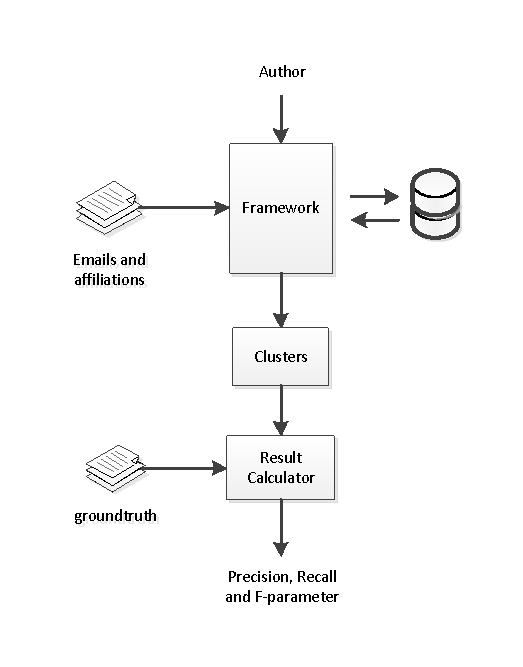
\includegraphics{./fig/testsetup.pdf}
	\label{fig:testsetup}
	\caption{A simplified overview of the testsetup starting with the author name and ending with the accuracy results.}
\end{figure}

The result calculator calculates the precision, recall and F measure as defined in \autoref{eq:prf}. Unless explicitly stated otherwise, when we refer to F measure, we mean the $F_{1}$ measure where recall and precision are equally important. These statistical values are calculated for each of the clusters from the groundtruth. 

\begin{equation}
	\label{eq:prf}
	\begin{array}{r c l}
		precision & = & \frac{\left|\left\{relevant~documents\right\} \cap \left\{retrieved~documents\right\}\right|}{\left|\left\{retrieved~documents\right\}\right|} \\
		recall & = & \frac{\left|\left\{relevant~documents\right\} \cap \left\{retrieved~documents\right\}\right|}{\left|\left\{relevant~documents\right\}\right|} \\
		F_{\beta} & = & ( 1 + \beta^{2} ) * \frac{precision * recall}{\beta^{2} * precision + recall} \\
	\end{array}
\end{equation}

If we denote the cluster of the groundtruth as $C_g$, then the calculated cluster from the graph the result calculator will $C_g$ compare with is given by 

\begin{equation}
	\label{eq:calccluster}
	\min_{\forall c \in calculated~clusters}{\left| C_g \setminus c \right|}
\end{equation}

In \autoref{eq:prf}, we use the terms relevant and retrieved documents. The explanations of these terms are given by the following definitions.

\begin{mydef}
	\textbf{Relevant documents} The publications from the cluster in the groundtruth
\end{mydef}

\begin{mydef}
	\textbf{Retrieved documents} The publications from the cluster calculated by the framework belonging to the cluster in the groundtruth, calculated in \autoref{eq:calccluster}
\end{mydef}

After calculating these statistical values for all the clusters in the groundtruth, the mean F measure is calculated to give us an idea of the accuracy for a given test.

\section{Results}

\subsection{Rules}

We have tested the influence of the different rules on the accuracy. For each of the families, we tested the same combination of rules in succession. The F measure for each of these combinations can be seen on \ref{fig:diff-rules}.

% bespreek figuur

\subsection{Weights}

We have tested different values for the weights allocated to each of the rules and also the value of \alpha which is used to determine if reclustering should occur. 

\subsection{Comparing to DBLP}

We have calculated the F measure for each of the families as they are divided on DBLP. They are depicted on \ref{table:f-dblp}. The divisions for "Turck" and "Mens" are completely correct, the other three are far less accurate with "Chen" having an astonishingly low F measure of $2.73\%$.

\begin{table}
	\centering
		\begin{tabular}{|c|c|c|c|c|c|c|c|}
			\hline
			& \bfseries{Turck} & \bfseries{Chen} & \bfseries{Woo} & \bfseries{Mens} & \bfseries{Johnson} & \bfseries{Mean} & \bfseries{Weighted} \\
			\hline
			\bfseries{DBLP} & 100.0\% & 87.5\% & 100.0\% & 2.7\% & 62.8\% & 70.6\% & 61.8\%\\
			\hline
			\bfseries{Framework} & & & & & & \\
		\end{tabular}
	\caption{Comparison of the F measures for the different families as they are divided on DBLP and as calculated by our framework. The last columns give the mean F measure and a weighted distribution based on the number of papers in each family.}
	\label{tab:f-dblp}
\end{table}